\chapter{Evaluation of cross sections}
\label{C:txs}


\section{Sextuple differential cross section}
The coordinates of the three-body system in the center of mass
reference frame are displayed in figure \ref{f:jacobi}
\todo[inline]{Agregar ac\'{a} la figura }
%
\begin{figure}[!htb]
    \centering
% \includegraphics[width=5.7cm,clip,bb =17 455 578 825]{jacobi}
\vspace{.5cm}
\caption{Jacobi coordinates. \label{f:jacobi}}
\end{figure}

The momenta associated to these pairs will be denoted
$\bm{k}_{j},\bm{K}_{j}$ while $\bm{k}, \bm{K}$ and $\bm{K}_{R}$ are the
the momenta of the electron, the projectile and the recoil-ion in the
laboratory coordinate system.

The sextuple differential cross section as a function of any two pairs
of Jacobi momenta is
%
\begin{equation}\label{Q:TDCS}
\frac{d \sigma}{d \bm{k}_{j} \, d \bm{K}_{j}} = \frac{(2
\pi)^{4}}{v} | t_{if}| ^{2} \delta \left( E_{i} -
\frac{K_{j}^{2}} {2 \mu_{j}} - \frac{k_{j}^{2}}{2 m_{j}}\right)
\end{equation}
%
where the transition matrix element is defined by $t_{if} = \langle
\Psi^{+}_{f} | V_{i} |  \Phi_{i} \rangle$.

From this equation we'll calculate the different lower-differential
cross sections.

\section{Quintuple (Triple) differential cross sections}

We are interested in different ``triple'' differential cross
sections\footnote{They are really quintuple differential with only 4
relevant variables} (TDCS). We'll quote the TDCS as a function of
different quantities.

\subsection{As a function of $Q,E_{k},\Omega_{k},
\varphi_{k\,Q}$}

The definition of the angles is given in figure \ref{f:coord}

\begin{figure}[!htb]
    \centering
%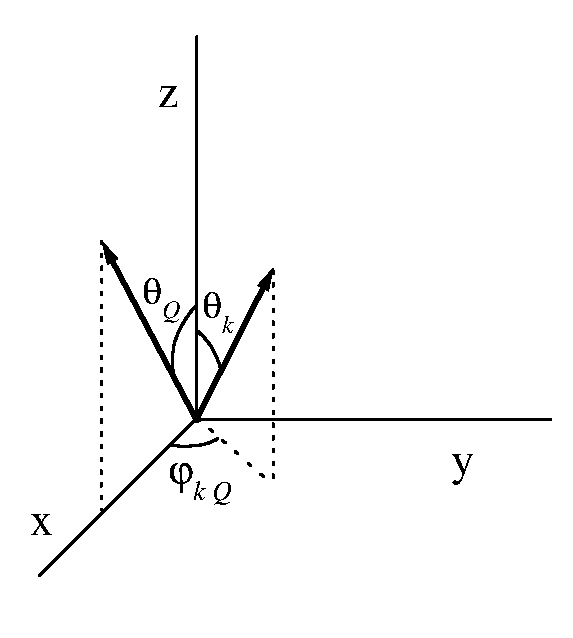
\includegraphics[height=7.5cm,clip,bb =55 495 309 760]{coord}
\caption{Definition of angles and planes used. \label{f:coord}}
\end{figure}

\begin{eqnarray} \label{Q:tdcs1}
\frac{d\sigma}{d E_{k} d\Omega_{k}d Q} &=&  m k \int
\frac{d\sigma}{d \bm{k} d \bm{Q} } d \Omega_{Q} \\
&=& m k \frac{(2 \pi)^{4}}{v}\int | t_{if}|^{2} \delta\left(
E_{i}-E_{f} \right) 2 \pi \, Q^{2} \, \sin \theta_{Q}\, d
\theta_{Q}\nonumber \\
&=& m k \frac{(2 \pi)^{5}\, Q^{2}}{v}\int | t_{if}| ^{2}
\delta\left(E_{i} - \frac{K^{2}_{j}} {2 \mu_{j} } - \frac{k^{2}_{j}}{2
m_{j} }\right) \sin \theta_{Q} \ d \theta \nonumber
\end{eqnarray}

  \noindent
Inserting $\bm{k}_{N}, \bm{K}_{N}$ as a function of $\bm{k}, \bm{Q}$ we
get for the argument of the delta function

\begin{equation}\label{Q:delta-kKN}
E_{i} - \left( \frac{K^{2}_{N}} {2 \mu_{N} } + \frac{\left| m_N \bm{v}
- \bm{Q} + (m_N/M_T) \bm{k} \right| ^{2}}{2 m_N }\right)
\end{equation}

  \noindent
Now, defining
\begin{equation}\label{Q:p-Qk}
\fbeq{ \bm{p} = (m_{N}/M_{T}) \bm{k} + m_{N} \bm{v}\,,}
\end{equation}
%
the conservation of the energy may be rewritten as
%
\begin{equation}\label{Q:Energ-conse-kQ}
E_{i} = \frac{K^{2}_{N}} {2 \mu_{N} } + \frac{| \bm{p} - \bm{Q}
| ^{2}}{2 m_{N}} = \frac{K^{2}_{N}} {2 \mu_{N} } + \frac{p^{2}}{2
m_{N}} + \frac{Q^{2}}{2 m_{N}} - \frac{\bm{p} \cdot \bm{Q}}{m_{N}}
\end{equation}
%
where $\bm{p} \cdot \bm{Q} \ =  Q \ \left(  p_x \sin{\theta_{Q} + p_{z}
\cos \theta_{Q} } \right)$.

We are ready to perform the integral in \ref{Q:delta-kKN} in the way
\[
\int f(x) \delta (g(x)) d x = \sum_{x} \frac{f(x)}{|
g'(x)| } \,.
\]
%
In our case, by defining
%
\[
  \fbeq{
 P_o = \frac{m_{N}}{Q} \left( \frac{K^{2}_{N}} {2 \mu_{N} }+
\frac{p^{2}}{2 m_{N}} + \frac{Q^{2}}{2 m_{N}} - E_{i} \right)
  }
\]
%
 we get
\[
g(\theta_Q) = \frac{Q}{m_{N}}(-P_{o} + \bm{p} \cdot \hat{Q}) =
\frac{Q}{m_{N}}(P_{o} + p_{x} \sin{(\theta_{Q})} + p_{z}
\cos{(\theta_{Q})})
\]
%
and
%
\[
g'(\theta_{Q}) = \frac{Q}{m_N} \left( p_{x} \cos \theta_{Q}  - p_{z}
\sin \theta_Q \right) \, ,
\] 
%
then the TDCS is given by
\begin{equation}\label{Q:5xsEkWkQ}
\fbeq{ \frac{d\sigma}{d E_{k} d\Omega_{k}d Q} =   \frac{(2
\pi)^{5} m k m_N\, Q}{v } \frac{ | t_{if}| ^{2}}{| p_{x}
\cot{\theta_Q} - p_{z} | }}
\end{equation}

Here $\theta_Q$ is the solution of the delta's argument $g(\theta_Q) =
0$. Explicitly,
$$
0 =  \bm{p} \cdot \hat{Q} - P_{o} =  p_{x} \sin{(\theta_{Q})} + p_{z}
\cos{(\theta_{Q})}  - P_{o} \nonumber \, .
$$
%
Then
%
\begin{eqnarray*}
&& \left( p_{z} -P_{o} \omega \right)^{2} = \left(- p_{x} \sqrt{(1
- \omega^{2})}\right)^2 \nonumber \\
&& P_{o}^{2} +  p_{z}^{2} \omega^{2} - 2 P_{o} p_{z} \omega = p_{x}^{2}
\left( 1 - \omega^{2}\right) \nonumber \\
\Rightarrow && (P_{o}^{2} - p_{x}^{2}) - 2 P_{o} p_{z} \; \omega +
(p_{z}^{2} + p_{x}^{2}) \; \omega^{2} = 0
  \, ,
\end{eqnarray*}
%
whose solutions are\footnote{Writing the result in this form, only the
`+' sign is valid. The `-' sign would be the correct result for
$\varphi_{k\,Q}' =2 \pi - \varphi_{k\,Q}$ such that
$\cos{\varphi_{k\,Q}}=\cos{\varphi_{k\,Q}'}$, but not for
$\varphi_{k\,Q}$.}
%
$$
\fbeq{\cos{(\theta_Q)}\, = \, \omega = \frac{P_{o} p_{z} {\pm} p_{x} \,
\sqrt{( p_{x}^{2} + p_{z}^{2} - P_{o}^{2} )}}{p_{x}^{2} + p_{z}^{2}}
\,} .
$$

\subsection{TDCS as a function of $\theta_{K}$, $E_{k}, \theta_{k}$
and $\varphi_{kK}$}

$$
\frac{d\sigma}{d E_{k} d\Omega_{k}d \Omega_{K}} = m k
\frac{(2 \pi)^{4}}{v}\int | t_{if}| ^{2} K^{2} \delta\left(
\frac{p^{2}_{N}} {2 m_{N} } - \frac{| \bm{K} - \bm{p}| ^{2}}{2
m_{N} }\right) \ d K
$$
%
with
\begin{equation}\label{Q:pN-defin}
    \fbeq{
p_{N} = \sqrt{2m_{N}\left( E_{i} - \frac{K_{N}^{2}}{2 \mu_{N}} \right)}
    }
\end{equation}
%
and
\begin{equation}\label{Q:p-defin}
   \fbeq{
\bm{p} = \left( m_{N}/M_{T}\right) \left(M_{P} \bm{v} - \bm{k} \right)
\, . }
\end{equation}
%
Then, we have
$$
 g(K) = \frac{-1}{2 m_{N}}\left( K^{2} + p^{2} - p_{N}^{2} - 2 \bm{K}
\cdot \bm{p} \right)
$$
and
$$
  g'(K) = \frac{- K + \bm{p} \cdot \hat{K}}{m_{N}} \,.
$$
%
The cross section is given by
\begin{equation}\label{Q:tdcsK}
    \fbeq{
\frac{d\sigma}{d E_{k} d\Omega_{k}d \Omega_{K}} = m k
\frac{(2 \pi)^{4}}{v} \, \frac{m_{N} K^{2}}{| K - \bm{p} \cdot
\hat{K}| } \, | t_{if}| ^{2}
    }
\end{equation}
%
where, by energy conservation,
\begin{equation}\label{Q:K-kQ}
\fbeq{K = \bm{p} \cdot \hat{K} {\pm} \sqrt{\left( \bm{p} \cdot \hat{K}
\right)^{2} + p_{N}^{2} - p^{2}} \,.
    }
\end{equation}

\subsection*{Approximated expressions}

When there is a large asymmetry between the electron and target mass
($m/M_{T} \ll 1$), $\bm{p} \approx m_N \bm{v}$ and the TDCS is given by
\begin{equation}\label{Q:5xsEkWkQapp}
\fbeq{ \frac{d\sigma}{d E_{k} d\Omega_{k}d Q} = \frac{(2
\pi)^{5} m k \, Q}{v^{2}} | t_{if}| ^{2}}
\end{equation}
%
where, for small values of $Q$, the polar angle is given by
$$
\cos{\theta_{Q}} \approx \frac{P_{o}}{m_{N} v} \ll 1 \, .
$$

The projectile scattering angle is \emph{approximately} proportional to
the transferred momentum by $\theta_{K} = Q/K$ ($K \approx M_{P} v$ is
the final projectile momentum). Then the TDCSs are simply related
$$
\frac{d\sigma}{d E_{k} d\Omega_{k}d \Omega_K} \approx
\frac{(M_{P} v)^{2}}{2 \pi \, Q} \frac{d\sigma}{d E_{k}
d\Omega_{k}d Q}
$$



\subsection{TDCS as a function of electron and transferred
momenta $\bi{k}$, $Q_{\parallel }, \bi{Q}_{\perp}$}

$$
\frac{d \sigma}{d \bm{k} d Q_{\parallel }} = \frac{(2
\pi)^{5}}{v} \int_{0}^{\infty} Q_{\perp} d Q_{\perp} |
t_{if}^{2}|  \; \delta \left( E_{i} - \frac{K_{j}^{2}}{2 \mu_{j}} -
\frac{k_{j}^{2}}{2 m_{j}}\right)
$$
%
By using
$$
  \fbeq{
\bm{p}= m_{N} \left( \bm{k}/M_{T} + \bm{v} \right)
  }
$$
%
as defined in \ref{Q:p-Qk} and
$$
p_{N} = \sqrt{2m_{N}\left( E_{i} - \frac{K_{N}^{2}}{2 \mu_{N}} \right)}
$$
%
we get for the argument of the delta function
%
$$
g(Q_{\perp}) = \frac{p_{N}^{2} - | \bm{p}- \bm{Q}| ^{2}}{2 m_{N}}
= \frac{p_{N}^{2} - p^{2} - Q^{2} + 2 \bm{p}\cdot \bm{Q}}{2 m_{N}}
$$
%
and then
$$
g'(Q_{\perp}) = \frac{1}{m_{N}}\left( - Q_{\perp} + \bm{p}_{\perp}
\right) \, .
$$

The TDCS is given by
%
\begin{equation}\label{Q:tdcsqpar}
  \fbeq{
\frac{d \sigma}{d \bm{k} d Q_{\parallel }} = \frac{(2
\pi)^{5}}{v} \frac{Q_{\perp} \, m_{N}}{| p_{\perp}- Q_{\perp} | }
\; | t_{if}| ^{2} }
\end{equation}
%
where $Q_{\perp}$ is the solution of a quadratic equation with
coefficient
$$
  \fbeq{
a=1\;, \quad b= - 2 p_{\perp} \;, \quad c= - \left( p_{N}^{2} - p^{2} -
Q_{\parallel }^{2} + 2 p_{\parallel } Q_{\parallel } \right)
  }
$$
%
given by
%
\begin{equation}\label{Q:qperp}
  \fbeq{
Q_{\perp} =  p_{\perp} {\pm} \sqrt{p_{\perp}^{2} + p_{N}^{2} - p^{2} -
Q_{| }^{2} + 2 p_{\parallel } Q_{\parallel }}
    }
\end{equation}
%
where only the `+' sign is valid. In particular, when $m/M_{T} \ll 1$
(atomic or molecular target), the perpendicular component of $\bm{p}$
is very small and
$$
Q_{\perp} \approx \sqrt{p_{N}^{2} - (m_{N} v)^{2} - Q_{\parallel
}^{2}} \,.
$$

The TDCS as a function of $Q_{\perp}$ is
%
\begin{equation}\label{Q:5xskQperp}
\frac{d \sigma}{d \bm{k} \, d \bm{Q}_{\perp}} = \frac{1}{2 \pi
Q_{\perp}} \frac{d \sigma}{d \bm{k} d Q_{\perp}} = \frac{(2
\pi)^{4}}{v} \, \int | t_{if}| ^{2} \; \delta \left( g(Q_{|
| }) \right) d Q_{\parallel }
\end{equation}
%
where, as before,
%
$$
g(Q_{\parallel }) = \frac{p_{N}^{2} - p^{2} - Q^{2} + 2 \bm{p}\cdot
\bm{Q}}{2 m_{N}} \, .
$$
%
The TDCS are then given by
\begin{equation}\label{Q:tdcsperp}
  \fbeq{
\frac{d \sigma}{d \bm{k} \, d \bm{Q}_{\perp}} = \frac{(2
\pi)^{4}}{v} \, \frac{m_{N}}{| p_{\parallel }- Q_{\parallel } |
}| t_{if}|^{2}
  }
\end{equation}
%
and
\begin{equation}\label{Q:tdcsperp1}
  \fbeq{
\frac{d \sigma}{d \bm{k} \, d Q_{\perp}} = \frac{(2
\pi)^{5}}{v} \, \frac{m_{N} Q_{\perp}}{| p_{\parallel }- Q_{|
| } | }| t_{if}| ^{2}
  }
\end{equation}
%
where $Q_{\parallel}$ the solution of a quadratic equation with
%
$$
  \fbeq{
a=1\;, \quad b= - 2 p_{\parallel } \;, \quad c= - \left( p_{N}^{2} -
p^{2} - Q_{\perp}^{2} + 2 p_{\perp} Q_{\perp} \right)
  }
$$
\begin{equation}\label{Q:qpar}
  \fbeq{
Q_{\parallel } =  p_{\parallel } {\pm} \sqrt{p_{\parallel }^{2} +
p_{N}^{2} - p^{2} - Q_{\perp}^{2} + 2 p_{\perp} Q_{\perp}}
    }
\end{equation}

\noindent
 The energy conservation can be rewritten by using the value of the
initial energy $E_{i}=\mu_{T} v^{2}/2 \, \varepsilon_{i}$. We obtain:

\begin{equation}\label{Q:EC1}
\bm{Q} \cdot \bm{v} + \frac{\bm{Q}\cdot \bm{k}}{M_{T}} - \frac{Q^{2}}{2
m_{N}} + \varepsilon_{i} - \frac{k^{2}}{2 m_{T}} = 0
\end{equation}
%
Then, $Q_{\parallel }$ can be obtained from a quadratic equation with
$$
a=\frac{1}{2 m_{N}} \, , \qquad b= -\left( v + \frac{k_{\parallel
}}{M_{T}} \right) \, , \qquad c= \frac{Q^{2}_{\perp}}{2 m_{N}} -
\frac{\bm{k}_{\perp} \cdot \bm{Q}_{\perp}}{M_{T}} - \varepsilon_{i} +
\frac{k^{2}}{2 m_{T}}
$$

\subsection{As a function of $ E_{k}, \theta_{k}, \varphi_{k,K_{R}},\theta_{K_{R}}$}

As in equation \ref{Q:tdcs1}, the cross section is given by

\begin{eqnarray} \label{Q:tdcs2}
\frac{d\sigma}{d E_{k} d\Omega_{k}d \Omega_{K_{R}}} &=& m k
\int
\frac{d\sigma}{d \bm{k} \, d \Omega_{K_{R}} } d K_{R} \\
&=& m k \frac{(2 \pi)^{4}}{v}\int | t_{if}| ^{2}
\delta\left(E_{i} - \frac{K^{2}_{j}} {2 \mu_{j} } - \frac{k^{2}_{j}}{2
m_{j} }\right) \, d K_{R} \, . \nonumber
\end{eqnarray}
%
Again we'll use the $(\bm{k}_N,\bm{K}_N)$ pair in the energy
conservation,
$$
E_{i} = \frac{K^{2}_{N}} {2 \mu_{N} } + \frac{\left| m_N \bm{v} -
\bm{K}_R + (m_N/M_T -1) \bm{k} \right|^{2}}{2 m_N } = \frac{K^{2}_{N}}
{2 \mu_{N} } + \frac{\left| m_N \bm{v} - \bm{K}_R - (m_N/M_P)\, \bm{k}
\right| ^{2}}{2 m_N }
$$
%
and define a vector
$$
\fbeq{\bm{p}=m_{N}(\bm{v} - \bm{k}/M_P).}
$$
%
Thus, defining
$$
P_o = \sqrt{{2 m_N} \left( E_{i} - \frac{K^{2}_{N}} {2 \mu_{N} }-
\frac{p^{2}}{2 m_{N}} \right)}
$$
the argument of the cross section is
$$
g(K_{R}) = \frac{1}{2 m_{N}} \left( P_o^{2} - K_{R}^{2} + 2 K_{R} \,
\hat{K}_{R} \cdot \bm{p} \right)
$$
and the derivative
$$
g'(K_{R}) = \frac{1}{m_{N}} \left(K_{R} - \bm{p} \cdot \hat{K}_{R}
\right)
$$

Then, the cross section is given by
\begin{equation}\label{Q:5xsEkWkWR}
  \fbeq{
\frac{d\sigma}{d E_{k} d\Omega_{k}d \Omega_{K_{R}}} =
\frac{(2 \pi)^{4} m k m_N}{v } \frac{ | t_{if}| ^{2}}{|  K_{R}
- \bm{p} \cdot \hat{K}_{R} | }
    }
\end{equation}
%
where the value of the $K_{R}$ modulus is fixed by energy conservation
$g(K_{R})=0$. Explicitly\footnote{Only the + sign is valid because
$K_{R}$ is defined positive},

\begin{equation}\label{Q:KR-k}
  \fbeq{
K_{R} =  \bm{p}\cdot \hat{K}_{R} {\pm} \sqrt{\left( \bm{p}\cdot \hat{K}_{R}
\right)^{2} + P_o^2}
  }
\end{equation}
%
with
$$
\bm{p}\cdot \hat{K}_{R} = p_{x} \sin{\theta_{R}} + p_{z}
\cos{\theta_{R}}
$$

\newpage
\subsection{As a function of $\bi{k}$, $K_{R \perp}$ ($K_{R \parallel }$)}
Closely related to the usual presentation of COLTRIMS results are the
cross sections
\begin{equation} \label{Q:tdcsxsr0}
\frac{d \sigma}{d \bm{k} \, d K_{R \perp}} = \frac{(2
\pi)^{4}}{v} \,(2 \pi K_{R \perp}) \int d K_{R | }, \parallel
t_{if}\parallel ^{2} \delta \left( E_{i} - E_{f} \right)
\end{equation}
%
and
\begin{equation}\label{Q:5xskR}
\frac{d \sigma}{d \bm{k} \, d K_{R \parallel }} = \frac{(2
\pi)^{4}}{v} \, \int d \bm{K}_{R \perp} \, | t_{if}| ^{2}
\delta \left( E_{i} - E_{f} \right) \, .
\end{equation}


In particular, for the first of them (eq. \ref{Q:tdcsxsr0}), we write
the conservation of the energy as $g(K_{R \perp}) = 0$, with
$$
g(K_{R \perp}) = \frac{1}{2 m_{N}} \left( P_o^{2} - K_{R | }^{2}
  - K_{R \perp}^{2} + 2 \bm{K}_{R} \cdot \bm{p} \right)
$$
and then
$$
g'(K_{R \perp}) = \frac{1}{m_{N}} \left( p_{\parallel } - K_{R \parallel }
\right) \,
$$
where $\bm{p} = m_{N}\left( \bm{v} - \bm{k}/M_{P}\right)$.

The cross section can be written
\begin{equation}\label{Q:tdcsxyr}
  \fbeq{
\frac{d \sigma}{d \bm{k} \, d K_{R \perp}} = \frac{(2
\pi)^{5}\,m_{N} \, K_{R \perp}}{v} \, \frac{ | t_{if}| ^{2}
}{| p_{\parallel } - K_{R | }| }
  }
\end{equation}
%
where, by energy conservation, $K_{R | }$ is the solution of a
quadratic equation with
%
$$
  \fbeq{
a=1 \qquad,\quad b = -2 p_{\parallel } \qquad \mbox{and} \quad c= -
\left( P_{o}^{2} + 2 K_{R \perp} p_{\perp} - K_{R\perp}^{2} \right)
  }
$$

%%%%%%%%%%%%%%%%%%%%%%%%%%%%%%%%%%%%%%%%%%%%%%%%%%%%%%%%%%%%%%%%%%%%%%%

\subsection{As a function of $\bi{K}_{R}$, $Q_{R \perp}$($Q_{R | }$)}

The energy conservation equation can be written,

\begin{equation}\label{Q:EC2}
\bm{Q} \cdot \textbf{v} + \frac{\bm{Q}\cdot \bm{K}_{R | }}{m} -
\frac{Q^{2}}{2 m_{P}} + \varepsilon_{i} - \frac{K^{2}_{R}}{2 m_{T}} = 0
\ .
\end{equation}

\noindent Taking into account the symmetry between $m$ and $M_{T}$, the
result is the same that for $d\sigma/d \bm{Q}_{\perp} d
\bm{k}$ but exchanging the role of electron and target-ion.

\subsection{As a function of $E_{k}$, $\theta_{R}$,
$\varphi_{Q,R}$, $Q_{\perp}$: { \texttt{Approximated expressions}}}

We calculate this TDCS as

$$
\frac{d\sigma}{d Q_{\perp} d E_k d \varphi_{Q,R} d
\theta_{K_{R}}} = \mathcal{J}_{o} \ \frac{K_{R}^{2}}{k/m} \,
\frac{d\sigma}{d Q_{\perp} d \bm{K}_{R}}
$$
%
where the Jacobian of the transformation is defined as
$$
\mathcal{J}_{o} = \frac{\partial \left( Q_{\perp}, \Omega_{\bm{K}_{R}}
, \ k \; \right) }{\partial \left( Q_{\perp}, \Omega_{\bm{K}_{R}} ,
K_{R} \right)} \ .
$$

In order to evaluate the Jacobian we write
%
\begin{equation}\label{Q:k-KR}
k^{2} = | \bm{Q} - \bm{K}_{R}| ^{2} = Q^{2} + K_{R}^{2} - 2 K_{R}
\left( Q_{\parallel } \cos{\theta_{K_{R}}} + Q_{\perp}
\sin{\theta_{K_{R}}} \cos{\varphi_{Q,R}}\right).
\end{equation}
%
Differentiating implicitly we find,

$$
\left( \frac{\partial K_{R}}{\partial k }\right)_{Q_{\perp},\,
  \Omega_{K_{R}}} =
\frac{ k - \left( Q_{\parallel } - K_{R} \cos{\theta_{K_{R}}}
\right)\displaystyle{ \left( \frac{\partial Q_{\parallel }}{\partial k
}\right)_{Q_{\perp},\, \Omega_{K_{R}}}}} {K_{R}- Q_{\parallel }
\cos{\theta_{K_{R}}} - Q_{\perp} \sin{\theta_{K_{R}}}
\cos{\varphi_{Q,R}} }
$$

\noindent
Here the magnitude of the recoil momentum is the solution of the second
order equation \ref{Q:KR-k}, with coefficients
$$
a=1 \quad  , \qquad b=-2 \left( Q_{\parallel } \cos{\theta_{K_{R}}} +
Q_{\perp} \sin{\theta_{K_{R}}} \cos{\varphi_{Q,R}}\right) \quad ,
\qquad c = Q^{2} - k^{2}
$$

  \noindent
where, in the approximation of heavy masses for the target and the
projectile, we have
$$
Q_{\parallel } = \frac{k^{2}/2m + | \varepsilon_{i}| }{v} \qquad
\qquad \Rightarrow \qquad \left( \frac{\partial Q_{\parallel
}}{\partial k }\right)_{Q_{\perp},\, \Omega_{K_{R}}} = \frac{k}{mv}
$$

\subsection{As a function of the P-e center of mass momentum}
\label{S:as-function-p}
Here we derive the cross section in terms of the pair of relative momenta: $(\bm{k}_{P}, \bm{k}_{P,cm})$, where $\bm{k}_{P,cm}$ is the momentum of the center of mass of the projectile-electron system.
From momentum conservation, we have $M_{P} \bm{v} = \bm{k}_{P,cm} + \bm{K}_{R}$, then:
$$
\bm{k}_{P,cm}= \bm{K}_{P} + \mu_{P}\frac{M_{P}}{M_{T}}\, \bm{v}
$$
We are interested in the following cross section:
$$
\frac{d \sigma}{d \bm{k}_{P} d \hat{k}_{P,cm}} = \frac{(2 \pi)^{4}}{v} \int |t_{if}|^{2} \delta \left( \frac{p_{p}^{2}}{2 m_{P}} - \frac{|\bm{k}_{P,cm} - \bm{p}|^{2}}{2 \mu_{P}} \right)
$$
%
where 
$$
p_{p}= \sqrt{2 \mu_{P}(E_{i}-\frac{k_{P}^{2}}{2 m_{P}})} \quad,\qquad \bm{p}=  \mu_{P}\frac{M_{P}}{M_{T}}\, \bm{v}
$$

Then, with the notation used above, we have
\begin{eqnarray*}
g(k_{P,cm})&=& - \frac{k_{P,cm}^{2}}{2 \mu_{P}} + k_{P,cm}\frac{\hat{k}_{P,cm} \cdot \bm{p}}{\mu_{P}} + \left( \frac{p_{P}^{2}}{2 \mu_{P}} - \frac{p^{2}}{2 \mu_{P}}\right) \\
g'(k_{P,cm})&=& \frac{1}{\mu_{P}}\left(  \hat{k}_{P,cm} \cdot \bm{p} - k_{P,cm} \right)
\end{eqnarray*}

Then, the desired cross section can be written as:
\begin{equation}\label{Q:xs-pe-cm}
  \frac{d \sigma}{d \bm{k}_{P} d \hat{k}_{P,cm}} = \frac{(2 \pi)^{4}\mu_{P} k^{2}_{P,cm} }{v}\frac{ |t_{if}|^{2}}{|\hat{k}_{P,cm} \cdot \bm{p} - k_{P,cm}|}
\end{equation}
%
where the magnitude of the vector is the solution of a quadratic equation with
$$
a=1 \quad  , \qquad b=-2 \left(\hat{k}_{P,cm} \cdot \bm{p} \right) \quad ,
\qquad c = p^{2} - p_{P}^{2}
$$

Observe that for light projectiles ($M_{P} \ll M_{T}$) the above expression may be simplified. The momentum $\bm{p}$ may be neglected in the denominator and the cross sections reads:
\begin{equation}\label{Q:xs-pe-cm-app}
  \frac{d \sigma}{d \bm{k}_{P} d \hat{k}_{P,cm}} \approx \frac{(2
    \pi)^{4}\mu_{P} k_{P,cm} }{v} \, |t_{if}|^{2} \quad ,  \qquad k_{P,cm}
  \approx p_{P}  
\end{equation}

The relation between the laboratory momenta and the relative and two-body center of mass momenta is
\[
\bm{k}= \bm{k}_{P} + \frac{m_{P}}{M_{P}}\bm{k}_{P,cm} \qquad \, \qquad
\bm{k}= -\bm{k}_{P} + \frac{m_{P}}{m}\bm{k}_{P,cm} 
\]
\section{Limit values of variables}
\label{S:Limit-value-varia}

Now we will obtain the minimum momentum transfer for a given value of
the electron momentum $\bm{k}$. We rewrite and simplify equation
\ref{Q:Energ-conse-kQ},

\begin{equation}\label{Q:Energ-conse-kQ-1}
p_{N} = \left| \bm{p} - \bm{Q} \right|
\end{equation}
%
where $p$ and $p_{N}$, given by equations \ref{Q:pN-defin} and
\ref{Q:p-defin}, depend on $\bm{k}$
\begin{eqnarray*}
\bm{p} &=& \left( m_{N}/M_{T}\right) \left(M_{P} \bm{v} - \bm{k}
\right)
\\
p_{N} &=& \sqrt{2m_{N}\left( E_{i} - \frac{K_{N}^{2}}{2
\mu_{N}} \right)}\, .
\end{eqnarray*}

This is the equation of a sphere centered in the momentum $\bm{p}$ and
with radius $p_{N}$. The minimum $Q$ corresponds to the vector that is
in the direction of $\bm{p}$ and the value is just the difference
between the center and the radius
%
\begin{equation}\label{Q:Qmin-k}
Q_{min} = |p_{N} - p| =  \sqrt{2m_{N}\left( E_{i} - \frac{K_{N}^{2}}{2
\mu_{N}} \right)} - \left( m_{N}/M_{T}\right) \left| M_{P} \bm{v} -
\bm{k} \right|
\end{equation}


\noindent To get it from the above equations we take squares in
equation \ref{Q:Energ-conse-kQ-1} to obtain a quadratic equation
$$
Q^{2} - 2 p\, Q \cos{\theta_{Q,p}} - \left( p_{N}^{2} - p^{2} \right) =
0 \, ,
$$
with positive solution
$$
Q = p\, \cos{\theta_{Q,p}} + \sqrt{(p\, \cos{\theta_{Q,p}})^{2} +
\left( p_{N}^{2} - p^{2} \right)} \, .
$$
%
The minimum value  given by \ref{Q:Qmin-k} corresponds to
$\theta_{Q,p}=\pi$.

The relation between the pairs $(\bm{k}_{P,cm}, \bm{k}_{P})$ and $(\bm{k},
\bm{Q})$ can be easily obtained by deriving the corresponding relations between
coordinates
\begin{eqnarray*}
  \bm{k}&=& \frac{m}{m+ M_{P}}\bm{k}_{P,cm} + \frac{m}{M_{P}}\bm{k}_{P} \\
  \bm{Q}&=& M_{P} \bm{v} - \frac{m}{m+ M_{P}}\bm{k}_{P,cm} + \bm{k}_{P}
\end{eqnarray*}


\section{Double differential cross sections}

The double differential cross section (DDCS) in the momentum of each
particle can be obtained by integrating the TDCS


\subsection{DDCS in the momentum $\bi{k}$ of the electron}

\begin{eqnarray*}
\frac{d \sigma}{d \bm{k}} &=& \int_{Q^{-}}^{Q^{+}} d Q
\int_{0}^{2 \pi} d \varphi \, \frac{d\sigma}{d \bm{k} \, d
Q d \varphi} \qquad  \qquad \mbox{with } \qquad Q^{\pm}= k_{N} {\pm} p
\\
&=& \int_{Q_{\parallel }^{-}}^{Q_{\parallel }^{+}} d Q_{\parallel
} \frac{d\sigma}{d \bm{k} \, d Q_{\parallel }}  \qquad \quad
\qquad \mbox{with }  \qquad \qquad Q^{\pm}_{\parallel } = k_{N} {\pm} p_{|
| }
\\
&=& 2 \pi \int_{0}^{Q_{\perp}^{+}} Q_{\perp} d Q_{\perp}
\frac{d\sigma}{d \bm{k} \, d \bm{Q}_{\perp}} \qquad \mbox{with
} \qquad\qquad Q_{\perp}^{\pm}= k_{N} {\pm} p_{\perp}
\end{eqnarray*}

We will now make explicit the evaluation given by the first of these
equations. The quintuple differential cross section


\subsection{Note on the evaluation of total cross sections}

The total cross section is obtained by integrating the single
differential cross section in electron energy. In the case of heavy
projectiles, the maximum electron energy is huge and, for every
practical use, indistinguishable from infinity. In the case of light
projectiles, while the recoil ion remains virtually at rest, its energy
can be neglected. Thus, the maximum electron energy would correspond to
the total energy ( electron-target binding energy subtracted to the
initial projectile kinetic energy). However, in a real calculation the
infinity limit is not practicable and the domain of integration must be
contained in a finite region. In many cases this limit will extend to a
few atomic units of energy. A good estimation of the energy becomes
numerically important when the integrand is expensive to compute. In
order to estimate the maximum electron energy which contributes
appreciable to the total cross section we use a classical
approximation.

The simplest, classical binary projectile-electron collision was
considered first by Thompson \parencite{Thomson1912PMp449}. This approximation
considers that the electron is initially at rest and that the target
nucleus only provides the binding energy. Within this approximation the
single differential cross section is given by
\begin{equation}\label{Q:Thomson}
\frac{d \sigma}{d (\Delta E)} = \frac{2 \pi Z_{P}^{2}}{m v^{2}
(\Delta E)^{2}}
\end{equation}
%
where
$$
\Delta E = I_{0} + E_{k}
$$
with $I_{0}=| \varepsilon_{i} | $. The total cross section in
this approximation is given by
$$
\sigma \equiv \sigma_{E_{0}} = \int_{I_{0}}^{E_{0}} \frac{d
\sigma}{d (\Delta E)} \,d (\Delta E) \,,
$$
where
$$
E_{0}= \frac{1}{2} (2 \,m_{P}\, v)^{2}
$$


\noindent Given the accuracy $\epsilon_{r}>0$, the upper limit
$E_{cut}$ in the integral in energy must verify
\[
  (\sigma - \sigma_{E_{cut}}) = \epsilon_{r} \, \sigma
\]

Inserting expression \ref{Q:Thomson} we obtain
\begin{equation}\label{Q:E-cut}
 \Delta E_{cut} = \frac{I_{0}/E_{0}}{\epsilon_{r} + I_{0}/E_{0}}\; E_{0}
\end{equation}

Thus, the cut energy is

$$
E_{cut} = I_{0}\left(\frac{1}{\epsilon_{r} + (I_{0}/E)} - 1 \right)
$$

\subsection{Change of variables}

The above estimation gives us an important clue. The dependence of the
single differential cross section with the electron energy (eq.
\ref{Q:Thomson}) can be used to improve numerical convergence. We write
the cross section as the product of a (unknown but smooth) function
$g(\Delta E)$ and $(\Delta E)^{-2}$
$$
\sigma = \int_{I_{0}}^{\Delta E_{cut}} \frac{d \sigma}{d (\Delta
E)}\, d (\Delta E) = \int_{I_{0}}^{\Delta E_{cut}} d (\Delta E)
\, \frac{g(\Delta E)}{(\Delta E)^{2}}
$$

Changing variables in the integral ($u=(\Delta E)^{-1}$), ($d u =
-(\Delta E)^{-2}\, d (\Delta E)$) we can write
$$
\sigma = \int_{1/\Delta E_{cut}}^{1/I_{0}}g(1/u) \; d u
$$
%
where $g(1/u)= (\Delta E)^{2} \, d \sigma / d (\Delta E)$.

%%% Local Variables: 
%%% mode: latex
%%% TeX-master: "mainxs"
%%% End: 
